\documentclass[a4paper,11pt]{article}

%%%%%%%%%%%%%%%%%%%%%%%%%%%%%%%%%
%            ATENÇÃO            %
% NÃO ALTERE AS LINHAS A SEGUIR %
%%%%%%%%%%%%%%%%%%%%%%%%%%%%%%%%%

\usepackage[brazil]{babel}
\usepackage{float,graphicx,graphics,amssymb,amsfonts,newlfont,indentfirst}
\usepackage[centertags]{amsmath}
\usepackage{fancyhdr}
\usepackage{ragged2e}
\usepackage{geometry}
\geometry{top=0cm,bottom=2cm,left=3cm,right=2cm}
\usepackage[normalem]{ulem}
\pagestyle{fancy}
\usepackage{url}
\usepackage{color}
\usepackage[font+=small,leftmargin=4cm,rightmargin=0cm,indentfirst=false]{quoting}
%\fancyfoot{} %retira número das páginas do rodapé
\renewcommand{\rmdefault}{ptm}
\renewcommand{\sfdefault}{ptm}
\renewcommand{\ttdefault}{ptm}

\lhead{ERMAC, Volta Redonda -- RJ, 2023}

\fancypagestyle{capa}{%
	\fancyhead{}%
	\rhead{\textit{Trabalho apresentado no ERMAC, Volta Redonda -- RJ, 2023.}%
	\vspace*{11pt}}%
}

\usepackage{mathptmx} % Fonte Times em fórmulas

\headheight 10mm
\oddsidemargin 2.0mm
\evensidemargin 2.0mm
\topmargin -10mm
\textheight 240mm
\textwidth 160mm
\headsep 5mm
\parindent 1mm


%%%%%%%%%%%%%%%%%%%%%%%%%%%%%
% MODIFIQUE DAQUI EM DIANTE %
%%%%%%%%%%%%%%%%%%%%%%%%%%%%%

% pacotes adicionais
%\usepackage{algorithm}

\begin{document}

\centering{{\Large{\bf Herramienta para la simulacion del crecimiento de tumores en diversas regiones del cuerpo humano en 3 dimensiones.}}

\begin{flushright}{\it
\vspace*{5mm}
Carlos Carret Miranda\\
Universidad de la Habana\\
carlos.carret@estudiantes.matcom.uh.cu

\vspace*{5mm}
\underline{ Reinaldo Rodríguez Ramos}\\
UFF/RJ e Univ. Havana/Cuba\\
email.autor2@yyy.zzz

\vspace*{5mm}
Nome completo do Autor 3\\
Instituição de vínculo do autor 2\\
email.autor3@yyy.zzz

% se necessário, adicione mais autores como nos blocos acima
}\end{flushright}


\setcounter{equation}{0} % NÃO modifique esta linha


\thispagestyle{capa}
\justifying{
{\noindent \bf Resumo: }{\small{%
	%RESUMO
	El cancer es una enfermedad que se caracteriza por el crecimiento descontrolado de células anormales en el cuerpo, es una enfermedad compleja y multifacética que ha desafiado a los investigadores y médicos durante décadas. La capacidad de visualizar y entender el crecimiento de los tumores puede proporcionar una valiosa comprensión de cómo se desarrolla y se propaga el cáncer, lo que puede llevar a mejoras significativas en el diagnóstico, tratamiento y prevención del cáncer. La herramienta de simulación tridimensional del crecimiento de tumores que estamos desarrollando es un paso importante en este sentido. Permite la visualización detallada del crecimiento de los tumores en diferentes partes del cuerpo humano, lo que puede proporcionar una valiosa comprensión de cómo se desarrolla y se propaga el cáncer. Además, la capacidad de esta herramienta para simular el crecimiento de tumores en diferentes partes del cuerpo significa que puede ser utilizada para estudiar una amplia gama de tipos de cáncer. 
}}

\vskip 0.2cm  % NÃO modifique esta linha


{\small{ %PALAVRAS-CHAVE
\noindent{\bf{Palavras-chave:}} Matemática Discreta. Otimização não linear. Navier-Stokes (entre 3 e 6 palavras-chave separadas por ponto)
}}
}

%%%%%%%%%%%%%%%%%%%%%%%%%%%%%
%%%%%%%%%%%%%%%%%%%%%%%%%%%%%

\section*{Introdução}

Os trabalhos aprovados para apresentação devem ser escritos, preferencialmente, na língua portuguesa, eventualmente, em língua inglesa, seguindo rigorosamente este modelo.


\section*{Submissão}

Observar os limites no número de páginas para cada categoria.

As Equações 1 e 2 são exemplos de formatação adequada para formas longas e curtas, respectivamente. A Equação de Navier-Stokes, juntamente com a equação de continuidade, em forma adimensional, são dadas por:

\begin{eqnarray}
\nonumber
\frac{\partial {\mathbf u}}{\partial t} + \nabla \cdot ({\mathbf uu}) &=& \frac{1}{\rho}\left\{-\nabla p + \frac{1}{Re}\,[\nabla \cdot (2 \mu S)] +\right.
\\
&& \left.+\frac{1}{Fr^2}\,\rho {\mathbf g} +
\frac{1}{We}\,\kappa \delta ({\mathbf x} - {\mathbf x}_f) {\mathbf n}\right\},
%\text{,}
\label{eq1}
\end{eqnarray}
e
\begin{equation}
\nabla \cdot {\mathbf u} = 0,
%\text{,}
\label{eq2}
\end{equation}
\normalsize
sendo $Re = \rho_{0}UL/ \mu_{0}$, $Fr = U/ \sqrt{Lg}$ e $We = \rho L U^2 /\sigma_{0}$ os números de Reynolds, Froude e Weber, respectivamente.

Tabelas, figuras e equações devem ser referenciadas com a enumeração em algarismos arábicos. Por exemplo, a Equação (\ref{eq1}) apresenta uma expressão longa em duas linhas, a Tabela \ref{fonts} indica os formatos de texto das diferentes partes do documento e a Figura \ref{niveis} mostra que os gráficos podem ser coloridos.


\begin{table}[h]
\caption{{\small Tipos de tamanhos de letra nas partes deste documento.}}\label{fonts}
\centering
\begin{tabular}{|c|c|c|c|}
\hline
{\bf Texto} & {\bf MS Word} & {\bf LaTeX} & {\bf Aparência} \\
\hline
título & 14pt & Large & \textbf{bold}\\
autor(es), instituição, e-mail & 11pt & normal & \textit{Itálico}\\
resumo, palavras-chave  &	10 pt	 & small  &	{\small normal}\\
texto principal	 &11 pt & normal & normal\\
\hline
\end{tabular}
\end{table}

O texto de legenda, para as tabelas e figuras, deve descrever os elementos principais das mesmas. Em LaTeX com figuras .jpg, usar pdflatex.

\begin{figure}[h]
\centering 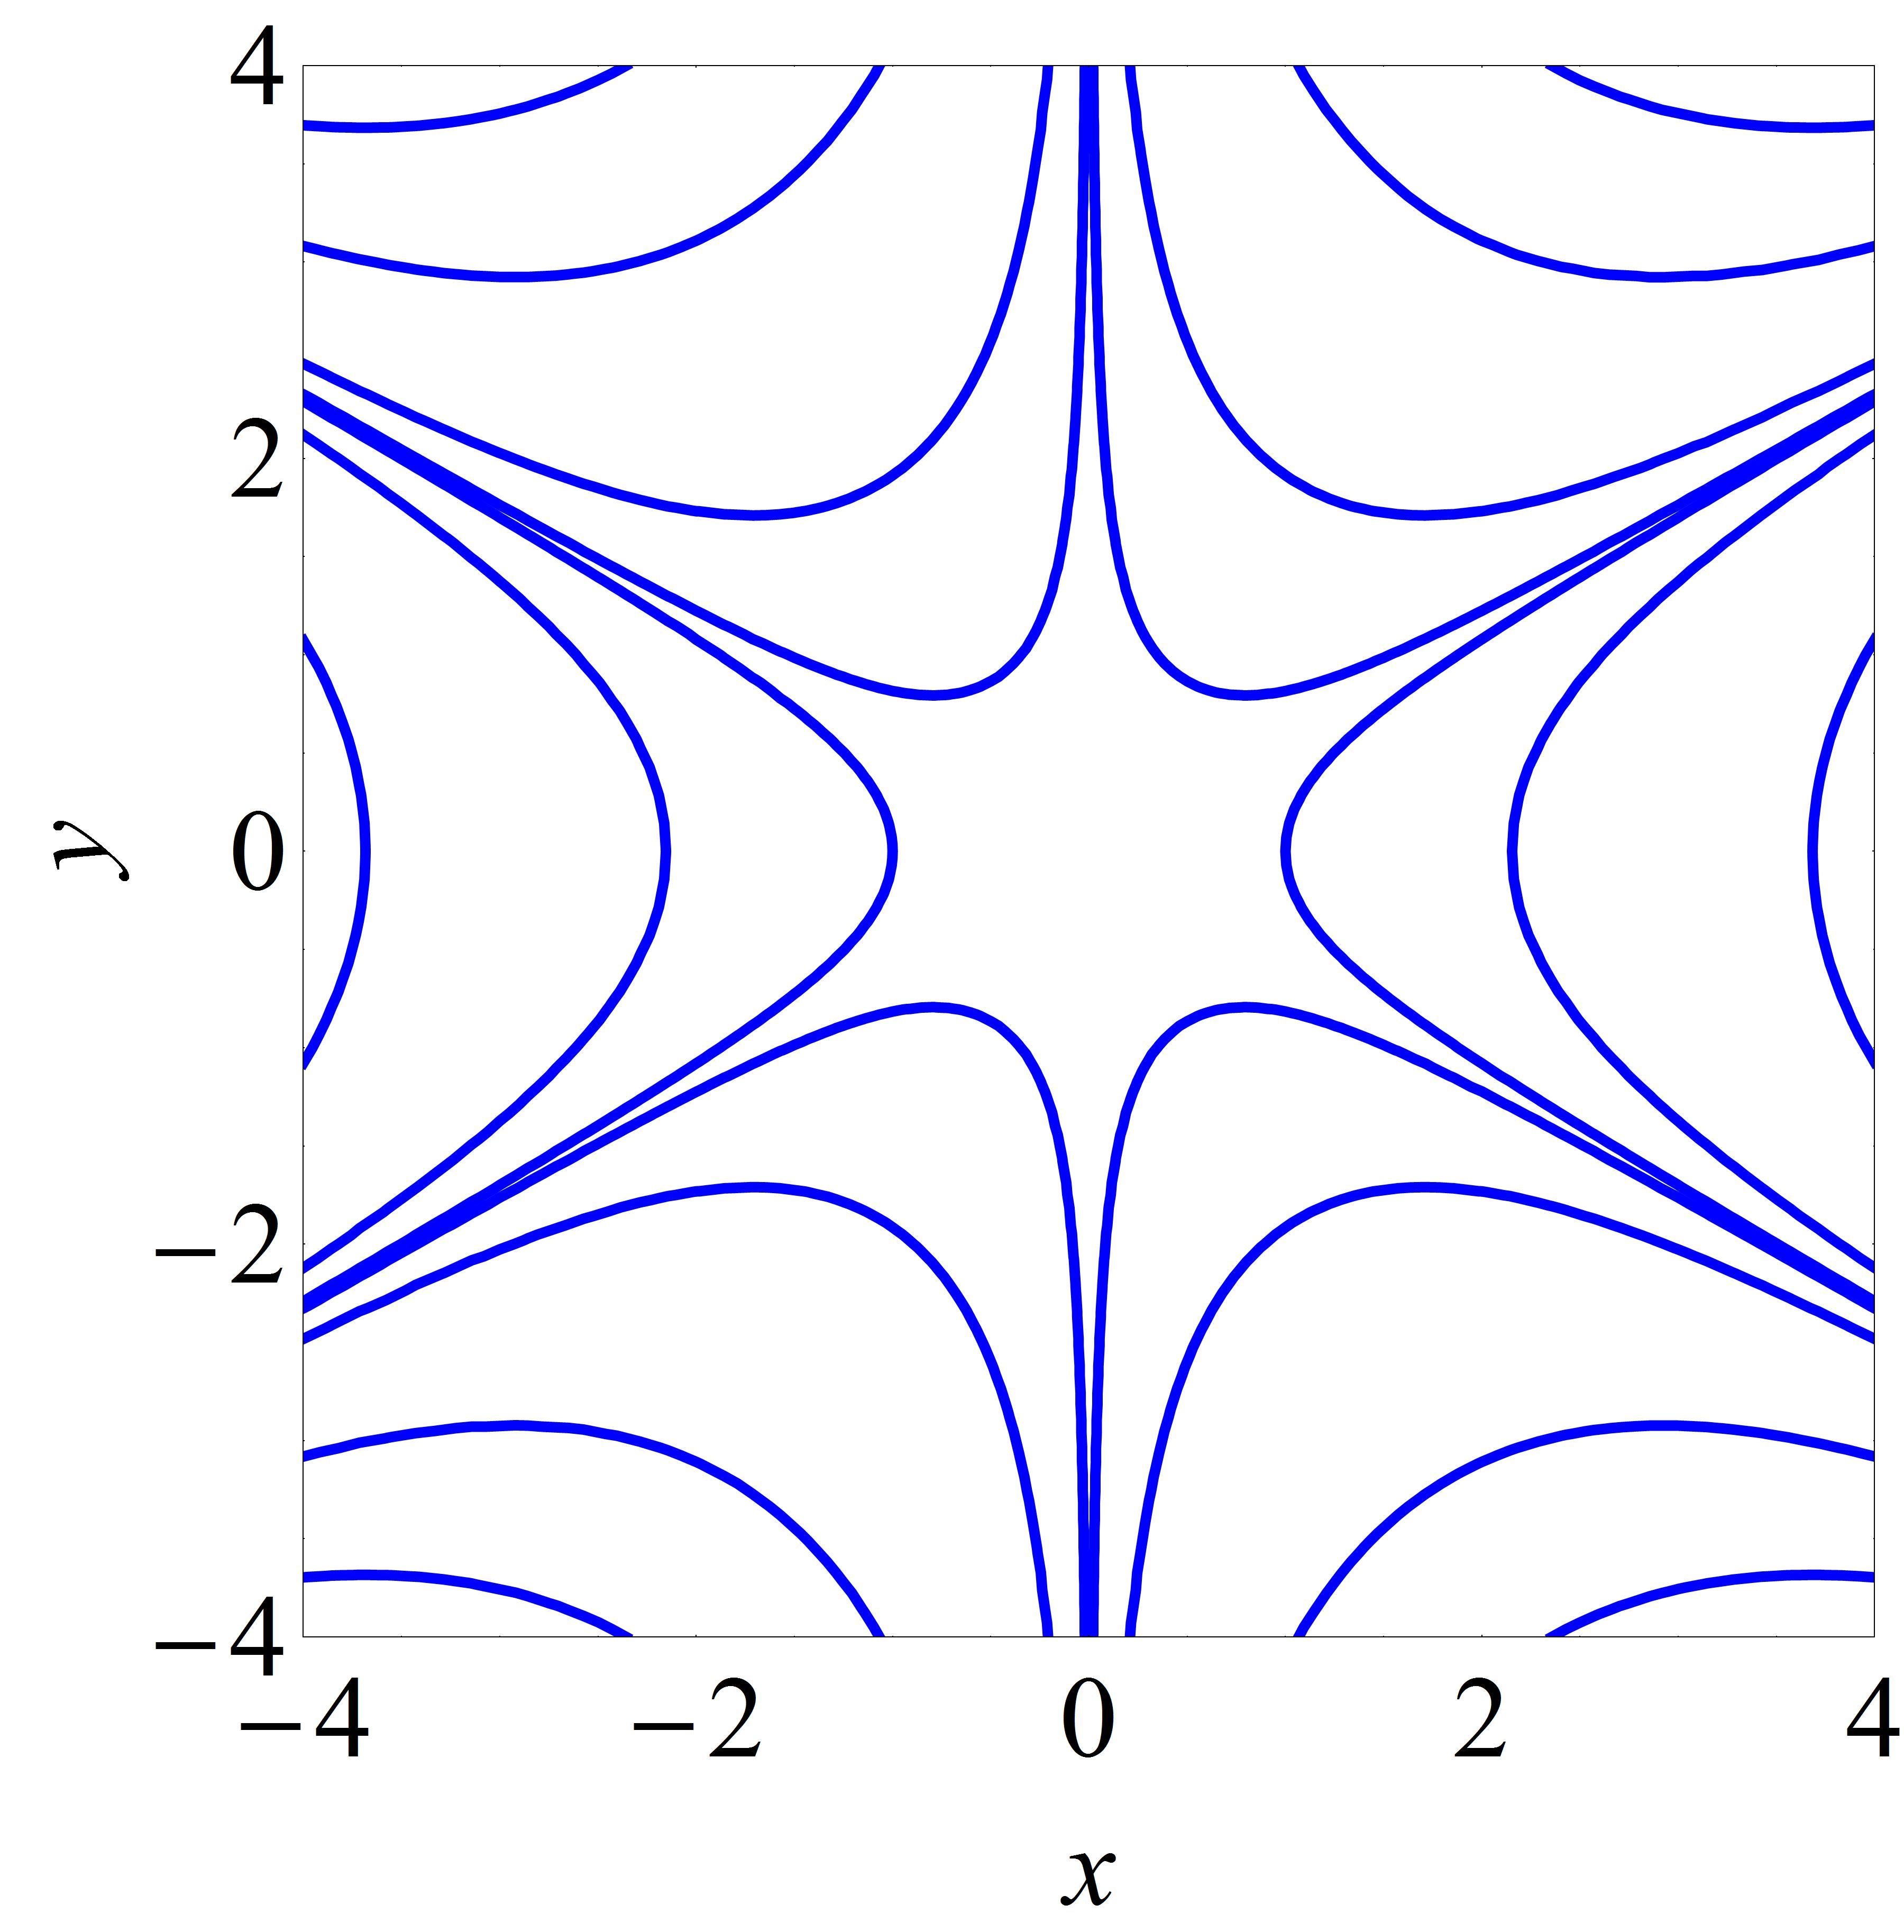
\includegraphics[height=4.5cm]{fig.jpg}\\
\caption{{\small Curvas de níveis da função $f(x,y)=x^3-3 x y^2$. }}
\label{niveis}
\end{figure}

{\bf IMPORTANTE:

O trabalho deve ser submetido via formulário que se encontra no site do evento.

Envie todos os arquivos necessários à produção do PDF em um único arquivo ZIP. Inclua o PDF compilado.
}


\section*{Seleção de trabalhos}

Os trabalhos submetidos, dentro do prazo estabelecido, serão enviados aos revisores do Comitê Científico. Com base nos pareceres do comitê, o trabalho poderá ser (1) aceito plenamente, (2) aceito sob a condição de que correções menores sejam feitas em curto prazo ou (3) rejeitado.


\section*{Citações}
Devem seguir as normas da ABNT NBR 10520. Nas citações, as chamadas pelo sobrenome do autor devem ser em letras maiúsculas e minúsculas e, quando estiverem entre parênteses, devem ser em letras maiúsculas.

Exemplos:

A ironia seria assim uma forma implícita de heterogeneidade mostrada, conforme a classificação proposta por Authier-Reiriz (1982).

\vskip 0.2cm
``Apesar das aparências, a desconstrução do logocentrismo não é uma psicanálise da filosofia [...]'' (DERRIDA, 1967, p. 293).

\vskip 0.2cm
a) As citações diretas, no texto, com mais de três linhas, devem ser destacadas com recuo de 4 cm da margem esquerda, espaço entre linhas simples e sem aspas, em fonte Times New Roman, tamanho 10.

\begin{quoting}
A teleconferência permite ao indivíduo participar de um encontro nacional ou regional sem a necessidade de deixar seu local de origem. Tipos comuns de teleconferência incluem o uso da televisão, telefone, e computador. Através de áudio-conferência, utilizando a companhia local de telefone, um sinal de áudio pode ser emitido em um salão de qualquer dimensão. (NICHOLS, 1993, p. 181).
\end{quoting}

\vskip 0.2cm
b) As citações diretas, no texto, de até três linhas, devem ser escritas entre ``aspas'' duplas e incorporadas ao texto.
Exemplos:
Barbour (1971, p. 35) descreve: ``O estudo da morfologia dos terrenos [...] ativos [...]''

\vskip 0.2cm
``Não se mova, faça de conta que está morta.'' (CLARAC; BONNIN, 1985, p. 72).

\vskip 0.2cm
Segundo Sá (1995, p. 27): ``[...] por meio da mesma `arte de conversação' que abrange tão extensa e significativa parte da nossa existência cotidiana [...]''

\vskip 0.2cm
c) Nas citações diretas, especificar no texto o ano de publicação e a(s) página(s) da fonte consultada. Estes dados devem ser colocados entre parênteses e separados por vírgula. Nas citações indiretas, a indicação da(s) página(s) consultada(s) é opcional, mas o ano de publicação da obra é obrigatório e deve estar entre parênteses.


\section*{Conclusões}

Em linhas gerais, as principais conclusões do trabalho.



\section*{Agradecimentos}

Os autores podem apresentar os agradecimentos a pessoas e instituições. Esta seção é OPCIONAL.



%%%%%%%%%%%%%%%%%%%%%%%%%%%%%
%%%%%%%%%%%%%%%%%%%%%%%%%%%%%

\section*{Referências}
{\color{red} A bibliografia deverá seguir o padrão da ABNT NBR 6023, separadas entre si por uma linha em branco, estar em \textbf{ordem alfabética pelo sobrenome do primeiro autor}, se necessário, usando-se, ainda, ordem cronológica, para trabalhos de um mesmo autor. Trabalhos dos mesmos autores, publicados no mesmo ano, devem ser listados utilizando-se a ordem alfabética do título do trabalho. Basicamente, as referências devem conter as iniciais dos nomes dos autores, sendo escrito, por extenso, apenas o último sobrenome. Seguem alguns exemplos:}


\begin{flushleft}

%Livro com até 3 autores:

GAUTSCHI, W. A survey of gauss-christoffel quadrature formulae. In: BUTZER, P.L.; FEHER, F. (Edit.). {\bf E. B. Christoffel: the influence of his work on mathematics and the physical sciences}. Basel; Boston: Birkhauser Verlag, 1981. p. 72-147.

\vskip 0.2cm
BRUNETTI, F. \textbf{Mecânica dos fluidos}. 2.ed. São Paulo:Pearson, 2005.

\vskip 0.2cm
JAIN, A.; ROSS, A.; NANDAKUMAR, K. \textbf{Introduction to Biometrics}. 1. ed. New York: Springer, 2001.

\vskip 0.2cm

%Livro com 4 autores ou mais:

ARENALES, M. et al. \textbf{Pesquisa Operacional}. Rio de Janeiro: Elsevier, 2006.

\vskip 0.2cm

%Artigo em periódico:

AVILA, A. Density of positive Lyapunov Exponents for $SL(2,\mathbb{R})$ cocycles. \textbf{Journal of the America Mathematical Society}, v. 24, n.4, p. 999-1014, 2011.

\vskip 0.2cm

KURODA, L. K. B. et al. Método da transformada diferencial generalizada no modelo fracionário de Malthus. \textbf{C.Q.D. - Revista Eletrônica Paulista de Matemática}, Bauru, v. 10, p. 68-78, dez. 2017. Edição Ermac. 

\vskip 0.2cm

%Trabalho em evento:

BRAYNER, A. R. A.; MEDEIROS, C. B. Incorporação do tempo em SGBD orientado a objetos. In: SIMPÓSIO BRASILEIRO DE BANCO DE DADOS, 9., 1994, São Paulo. \textbf{Anais...} São Paulo: USP, 1994. p. 16-29.

\vskip 0.2cm

%Dissertações e teses:

CHERRI, A.C. \textbf{Reaprendendo tópicos de cálculo diferencial com o auxilio de softwares matemáticos}. 2001. 154 f. Trabalho de Conclusão de Curso (Especialização) \textendash\ Faculdade de Ciências, UNESP, Bauru, 2001.

\vskip 0.2cm
DINIZ,G. L. \textbf{A mudança no habitat de populações de peixes: de rio a represa -- o modelo
matemático}. 1994. 90 f. Dissertação (Mestrado em Matemática Aplicada) \textendash\ Unicamp, Campinas, 1994.

\vskip 0.2cm
OLIVEIRA, E.L. \textbf{Torres de Extensões Abelianas
de grau primo ímpar não ramificado}.2015. 63f. Tese (Doutorado em Matemática) \textendash\ IBILCE/UNESP, São José do Rio Preto, 2015.

\vskip 0.2cm

%Homepages:

INTERNATIONAL GEOGEBRA INSTITUTE. Matemática dinâmica para se aprender e se ensinar. 2014. Disponível em: http://www.geogebra.org/cms. Acesso em: 17 dez. 2014.
\end{flushleft}

\end{document}
